\documentclass[20pt,landscape,a4paper,footrule]{foils}
\usepackage{zencurity-slides}


%
% Arrangement:	Penetration testing I - basale pentest metoder og introduktion

% Penetration testing IV - cryptography og cracking

% Kryptografi er en forudsætning for en stol del af vores IT-sikkerhed, men hvad er sikkert? Vi gennemgår forudsætningerne og nogle af de mest almindelige værktøjer til at sikre og knække kryptering. Vi bruger tidligere knækkede algoritmer som eksempler og udfra denne viden opnår vi erfaring som tillader os at vælge hvilke protokoller vi fremover vil benytte til at sikre os. Dette kursus sigter mod at deltagerne efterfølgende vælger de rigtige metoder og kryptering til at sikre systemer og data.

% * Password cracking
% * Wireless cracking / WPA cracking
% * Fuld disk kryptering - forudsætninger og eksempler på fejl
% * GPU og FPGA cracking
% * OpenSSL / LibreSSL - heartbleed som eksempel
% * Tilfældige tal og PRNG Debian
% * IPsec, OpenVPN og andre VPN teknologier, PPTP
% * OPsec
% sslyze
% sslscan
% john the ripper - de skal selv prøve

% Måske lave DMG de kan knække?
% Måske DNS walk the zone with DNSSEC
% Husk link til lets encrypt
\begin{document}

\mytitlepage
{Penetration testing IV\\pentest cryptography and cracking}

%\begin{alltt}
%\tiny
%\centerline{$Id: pentest-I-foredrag.tex,v 1.2 2007/10/04 12:17:42 hlk Exp $}
%\end{alltt}



\LogoOn

%\dagsplan


\slide{Goals for today}

\hlkimage{8cm}{Encrypt_all_the_things.png}

\begin{list1}
\item Introduce some common cryptographic protocols
\item Introduce some often used pentest tools in cryptography
\item Increase paranoia to appropriate levels \smiley
\item Reference some classics
\end{list1}

\slide{Generic advice}

Recommendations \hlkrightimage{5cm}{Encrypt_all_the_things.png}
\begin{list2}
\item Lock your devices, phones, tables and computers
\item Update software and apps
\item Do NOT use the same password everywhere
\item Watch out when using open wifi-networks
\item Multiple browsers: one for Facebook, and separate for home banking apps?
\item Multiple laptops? One for private data, one for work?
\item Think of the data you produce, why do people take naked pictures and SnapChat them?
\item Use pseudonyms and aliases, do not use your real name everywhere
\item Enable encryption: IMAP{\bf S} POP3{\bf S}
  HTTP{\bf S} TOR OpenPGP VPN SSL/TLS
\end{list2}


\slide{Stop watching us!}

\hlkimage{20cm}{access-now.png}

\slide{Appropriate paranoia}

\hlkimage{15cm}{paranoia-definition.png}

Source: google paranoia definition

\slide{Face reality}

From the definition:
\begin{quote}
suspicion and mistrust of people or their actions  {\bf without evidence or justification}.
"the global paranoia about hackers and viruses"
\end{quote}

\begin{list1}
\item It is not paranoia when:
\begin{list2}
\item Criminals sell your credit card information and identity theft
\item Trade infected computers like a commodity
\item Governments write laws that allows them to introduce back-doors - and use these
\item Governments do blanket surveillance of their population
\item Governments implement censorship, threaten citizens and journalist
\end{list2}
\end{list1}

\vskip 1cm
\centerline{You are not paranoid when there are people actively attacking you!}


\slide{Credit card fraud and identity theft statistics}

\hlkimage{19cm}{credit-card-fraud.png}

{\small Source:
\link{http://www.statisticbrain.com/credit-card-fraud-statistics/}}


\slide{Identity theft statistics}

\hlkimage{19cm}{identity-theft-stat.png}

{\small Source:
\link{http://www.statisticbrain.com/identity-theft-fraud-statistics/}}


\slide{Use protection - always}

\hlkimage{14cm}{protect-from-governments.jpg}
%{\LARGE Protecting yourself against criminals or the government is the same thing!}

\slide{A vulnerability can and will be abused}

What if I told you:

{\Large \bf Criminals will be happy to leverage backdoors created by government}

It does not matter if the crypto product has a weakness to allow investigations or the software has a backdoor to help law enforcement. Data and vulnerabilities WILL be abused and exploited.

Make sure to read \emph{Keys Under Doormats:
mandating insecurity by requiring government access to all data and communications}

\link{https://www.cl.cam.ac.uk/~rja14/Papers/doormats.pdf}

\link{http://savecrypto.org}


\slide{Why think of security?}

\hlkimage{8cm}{1984-not-instruction-manual.jpg}


\begin{quote}
	Privacy is necessary for an open society in the electronic age. Privacy is not secrecy. A private matter is something one doesn't want the whole world to know, but a secret matter is something one doesn't want anybody to know. Privacy is the power to selectively reveal oneself to the world. ~A Cypherpunk's Manifesto by Eric Hughes, 1993
\end{quote}

Copied from \link{https://cryptoparty.org/wiki/CryptoParty}

\slide{Starting the crypto journey}

Where do we start?

\hlkimage{6cm}{network-security-book-perlman9780137155880_s.jpeg}
\centerline{Private Communications in an Public World}

Very nice book listing our knowledge about main protocols in use on the internet today - even though the book is from 2002! Includes: IPsec, SSL/TLS, PGP, PKI, AES m.fl.

\slide{First advice}

\begin{list1}
\item Use technology
\item Learn the technology - read the freaking manual
\item Think about the data you have, upload, facebook license?! WTF!
\item Think about the data you create - nude pictures taken, where will they show up?
\begin{list2}
\item Turn off features you don't use
\item Turn off network connections when not in use
\item Update software and applications
\item Turn on encryption: IMAP{\bf S}, POP3{\bf S},
  HTTP{\bf S} also for data at rest, full disk encryption, tablet encryption
\item Lock devices automatically when not used for 10 minutes
\item Dont trust fancy logins like fingerprint scanner or face recognition on cheap devices
\end{list2}
\end{list1}

\slide{Chaosreader}

\hlkimage{5cm}{chaosreader1.jpg}
\hlkimage{20cm}{chaosreader2.png}
\begin{list1}
\item Simple but illustrative program
\item Read a pcap - packet capture into this tool chaosreader
\item Output HTML with nice index - usefull for quick demos
\item \link{http://chaosreader.sourceforge.net/}

\end{list1}

\slide{Big data example Moloch}

\hlkimage{16cm}{moloch-sessions.png}

Picture from \link{https://github.com/aol/moloch}\\
Be your own GCHQ ... capture all, index all, search all

\slide{Cryptography}


\begin{list1}
\item Cryptography or cryptology is the practice and study of techniques for secure communication
\item Modern cryptography is heavily based on mathematical theory and computer science practice; cryptographic algorithms are designed around computational hardness assumptions, making such algorithms hard to break in practice by any adversary
\item Symmetric-key cryptography refers to encryption methods in which both the sender and receiver share the same key, to ensure confidentiality, example algorithm AES
\item Public-key cryptography (like RSA) uses two related keys, a key pair of a public key and a private key. This allows for easier key exchanges, and can provide confidentiality, and methods for signatures and other services
\end{list1}

Source: \link{https://en.wikipedia.org/wiki/Cryptography}

\slide{Kryptografiske principper}

\begin{list1}
\item Algoritmerne er kendte
\item Nøglerne er hemmelige
\item Nøgler har en vis levetid - de skal skiftes ofte
\item Et successfuldt angreb på en krypto-algoritme er enhver genvej
  som kræver mindre arbejde end en gennemgang af alle nøglerne
\item Nye algoritmer, programmer, protokoller m.v. skal gennemgås nøje!
\item Se evt. Snake Oil Warning Signs:
Encryption Software to Avoid\\
\link{http://www.interhack.net/people/cmcurtin/snake-oil-faq.html}
\end{list1}

\slide{DES, Triple DES og AES}

\hlkimage{15cm}{images/AES_head.png}

\begin{list1}
\item DES kryptering baseret på den IBM udviklede Lucifer algoritme
  har været benyttet gennem mange år
\item Der blev i 2001 vedtaget en ny standard algoritme Advanced Encryption
  Standard (AES) som afløser Data Encryption Standard (DES)
\item Algoritmen hedder Rijndael og er udviklet
af Joan Daemen og Vincent Rijmen.
%\item \emph{Rijndael is available for free. You can use it for
%whatever purposes  you want, irrespective of whether
%it is accepted as AES or not.}
\item Se også \link{https://en.wikipedia.org/wiki/Advanced_Encryption_Standard}
\end{list1}


\slide{Formålet med kryptering}

\vskip 3 cm
\centerline{\hlkbig kryptering er den eneste måde at sikre:}
\vskip 3 cm
\centerline{\hlkbig fortrolighed}
\vskip 3 cm
\centerline{\hlkbig autenticitet / integritet}


%%% Local Variables:
%%% mode: latex
%%% TeX-master: "tcpip-security"
%%% End:


\slide{Secure protocols}

\begin{list1}
\item Securing e-mail
\begin{list2}
\item Pretty Good Privacy - Phil Zimmermann
\item OpenPGP = e-mail security
\end{list2}
\item Network sessions use SSL/TLS
\begin{list2}
\item Secure Sockets Layer SSL / Transport Layer Services TLS
\item Encrypting data sent and received
\item SSL/TLS already used for many protocols as a wrapper: POP3S, IMAPS, SSH, SMTP+TLS m.fl.
\end{list2}
\item Encrypting traffic at the network layer - Virtual Private Networks VPN
\begin{list2}
\item {\color{green}IPsec IP Security Framework, se også L2TP}
\item {\color{red} PPTP Point to Point Tunneling Protocol - dårlig og usikker, brug den ikke mere!}
\item OpenVPN uses SSL/TLS across TCP or UDP
\end{list2}
\end{list1}

\centerline{Note: SSL/TLS is not trivial to implement, key management!}

\slide{SSL og TLS}

\hlkimage{14cm}{ehandel-https.pdf}

\begin{list1}
\item Oprindeligt udviklet af Netscape Communications Inc.
\item Secure Sockets Layer SSL er idag blevet adopteret af IETF og kaldes
derfor også for Transport Layer Security TLS
TLS er baseret på SSL Version 3.0
\item RFC-2246 The TLS Protocol Version 1.0 fra Januar 1999
\item RFC-3207 SMTP STARTTLS
\end{list1}


\slide{SSL}

\begin{quote}
The 'S' in HTTPS stands for 'secure' and the security is provided by SSL/TLS. SSL/TLS is a standard network protocol which is implemented in every browser and web server to provide confidentiality and integrity for HTTPS traffic.
\end{quote}

\begin{list1}
\item Nu vi snakker om kryptering - SSL overalt?
\item Kan vi klare det på vores servere?
\pause
\item Google kan:\\
\link{http://www.imperialviolet.org/2010/06/25/overclocking-ssl.html}
\item Men alt for få gør det
\end{list1}
\pause
\centerline{Næste spørgsmål er så hvilke rod-certifikater man stoler på ...}



\slide{Heartbleed CVE-2014-0160}

\hlkimage{22cm}{heartbleed-com.png}

Source: \link{http://heartbleed.com/}

\slide{Heartbleed is yet another bug in SSL products}

\begin{alltt}
What versions of the OpenSSL are affected?
Status of different versions:

* OpenSSL 1.0.1 through 1.0.1f (inclusive) are vulnerable
* OpenSSL 1.0.1g is NOT vulnerable
* OpenSSL 1.0.0 branch is NOT vulnerable
* OpenSSL 0.9.8 branch is NOT vulnerable

Bug was introduced to OpenSSL in December 2011 and has been out
in the wild since OpenSSL release 1.0.1 on 14th of March
2012. OpenSSL 1.0.1g released on 7th of April 2014 fixes the bug.
\end{alltt}

\vskip 1cm
\centerline{It's just a bug - but a serious one}

\slide{Why is heartbleed different?}

\hlkimage{3cm}{heartbleed.png}
\begin{list1}
\item Great PR, name, web site, logo
\item OpenSSL is very widespread
\item OpenSSL has been criticized before
\item The spotlight is now on a lot of products, infrastructure
\item BOTH Open Source products and Proprietary products hurt by this
\item TL;DR\\ OpenSSL is everywhere and an example of our dependency on weak components
\end{list1}

\slide{Key points after heartbleed}

\hlkimage{16cm}{ssl-tls-breaks-timeline.png}
Source: picture source\\ {\footnotesize\link{https://www.duosecurity.com/blog/heartbleed-defense-in-depth-part-2}}
\begin{list2}
\item Writing SSL software and other secure crypto software is hard
\item Configuring SSL is hard\\
check you own site \link{https://www.ssllabs.com/ssltest/}
\item SSL is hard, finding bugs "all the time"
\link{http://armoredbarista.blogspot.dk/2013/01/a-brief-chronology-of-ssltls-attacks.html}
\item Rekeying is hard - slow, error prone, manual proces - Automate!
\item Proof of concept programs exist - good or bad?
\end{list2}

\slide{Proof of concept programs exist - good or bad?}

\centerline{Some of the tools released shortly after Heartbleed announcement}
\begin{list2}
\item \link{https://github.com/FiloSottile/Heartbleed} tool i Go\\
site \link{http://filippo.io/Heartbleed/}
\item \link{https://github.com/titanous/heartbleeder} tool i Go
\item \link{http://s3.jspenguin.org/ssltest.py} PoC
\item \link{https://gist.github.com/takeshixx/10107280} test tool med STARTTLS support
\item \link{http://possible.lv/tools/hb/} test site
\item \link{https://twitter.com/richinseattle/status/453717235379355649} Practical Heartbleed attack against session keys links til, \link{https://www.mattslifebytes.com/?p=533} og "Fully automated here "\\ \link{https://www.michael-p-davis.com/using-heartbleed-for-hijacking-user-sessions/}

\item Metasploit er også opdateret på master repo\\ \link{https://twitter.com/firefart/status/453758091658792960}\\
\link{https://github.com/rapid7/metasploit-framework/blob/master/modules/auxiliary/scanner/ssl/openssl_heartbleed.rb}
\end{list2}



\slide{Heartbleed hacking}

\begin{alltt}\footnotesize
  06b0: 2D 63 61 63 68 65 0D 0A 43 61 63 68 65 2D 43 6F  -cache..Cache-Co
  06c0: 6E 74 72 6F 6C 3A 20 6E 6F 2D 63 61 63 68 65 0D  ntrol: no-cache.
  06d0: 0A 0D 0A 61 63 74 69 6F 6E 3D 67 63 5F 69 6E 73  ...action=gc_ins
  06e0: 65 72 74 5F 6F 72 64 65 72 26 62 69 6C 6C 6E 6F  ert_order&billno
  06f0: 3D 50 5A 4B 31 31 30 31 26 70 61 79 6D 65 6E 74  =PZK1101&payment
  0700: 5F 69 64 3D 31 26 63 61 72 64 5F 6E 75 6D 62 65  _id=1&card_numbe
  0710: XX XX XX XX XX XX XX XX XX XX XX XX XX XX XX XX   r=4060xxxx413xxx
  0720: 39 36 26 63 61 72 64 5F 65 78 70 5F 6D 6F 6E 74  96&card_exp_mont
  0730: 68 3D 30 32 26 63 61 72 64 5F 65 78 70 5F 79 65  h=02&card_exp_ye
  0740: 61 72 3D 31 37 26 63 61 72 64 5F 63 76 6E 3D 31  ar=17&card_cvn=1
  0750: 30 39 F8 6C 1B E5 72 CA 61 4D 06 4E B3 54 BC DA  09.l..r.aM.N.T..
\end{alltt}

\begin{list2}
\item Obtained using Heartbleed proof of concepts - Gave full credit card details
\item "can XXX be exploited" - yes, clearly! PoCs ARE needed\\
without PoCs even Akamai wouldn't have repaired completely!
\item The internet was ALMOST fooled into thinking getting private keys from Heartbleed was not possible - scary indeed.
\end{list2}

\slide{Analysis of the heartbleed bug}

\begin{list2}
\item analyse af problemet i koden\\
{\small\link{http://blog.existentialize.com/diagnosis-of-the-openssl-heartbleed-bug.html}}
\item IDS regler Detecting OpenSSL Heartbleed with Suricata\\
{\small\link{http://blog.inliniac.net/2014/04/08/detecting-openssl-heartbleed-with-suricata/}}
\item god beskrivelse af hvordan man kan fixe hurtigere hvis man har automatiseret infrastruktur\\\link{https://www.getpantheon.com/heartbleed-fix}

\item Mange blogindlæg om emnet - eksempelvis\\
{\small\link{http://blog.fox-it.com/2014/04/08/openssl-heartbleed-bug-live-blog/} }

\item "nse script ssl-heartbleed.nse committed to nmap as rev 32798. "
\item You can now use Masscan to scan the whole internet for the Hearbleed vulnerability in under 6 minutes \link{https://twitter.com/jedisct1/status/453679529710460928}\\ og {\small\link{https://github.com/robertdavidgraham/masscan/commit/23497c448b0a1c7058e8443e5202e7bffcab4795}}
\end{list2}

\slide{Heartbleed Conclusions}

\begin{list1}
\item Nothing new, but more focus on problems?\\
Really is there something new in this?
\item Software has bugs - stay vigilant, implement defense in depth
\item Software need funding - especially software used in our critical systems
\item Security needs proof of concepts and open communication\\
Akamai fix that wasn't good enough!
\end{list1}

\vskip 2cm

\centerline{TL;DR Fund more security audits, stop using untested/unaudited software}


\slide{Weak DH paper}

\hlkimage{18cm}{weakdh-logjam.png}

Source: \link{https://weakdh.org/} and \\
\link{https://weakdh.org/imperfect-forward-secrecy-ccs15.pdf}

\slide{Audits}

\hlkimage{10cm}{crypto-cat.png}
\begin{list1}
\item Truecrypt audit\\
{\footnotesize\link{https://isecpartners.github.io/news/2014/04/14/iSEC-Completes-Truecrypt-Audit.html}}
\item Cryptocat audit\\
{\footnotesize\link{https://blog.crypto.cat/2013/02/cryptocat-passes-security-audit-with-flying-colors/}}
\end{list1}


%\slide{Improving your cryptography configurations}

\slide{Bettercrypto.org}

\hlkimage{20cm}{bettercrypto-nginx.png}
\begin{quote}
Overview

This whitepaper arose out of the need for system administrators to have an updated, solid, well researched and thought-through guide for configuring SSL, PGP, SSH and other cryptographic tools in the post-Snowden age. ... This guide is specifically written for these system administrators.
\end{quote}

\link{https://bettercrypto.org/}


\slide{sslscan}

\begin{alltt}\small
root@kali:~# sslscan --ssl2 web.gratisdns.dk
Version: 1.10.5-static
OpenSSL 1.0.2e-dev xx XXX xxxx

Testing SSL server web.gratisdns.dk on port 443
...
  SSL Certificate:
Signature Algorithm: sha256WithRSAEncryption
RSA Key Strength:    2048

Subject:  *.gratisdns.dk
Altnames: DNS:*.gratisdns.dk, DNS:gratisdns.dk
Issuer:   AlphaSSL CA - SHA256 - G2
\end{alltt}

Source:
Originally sslscan from http://www.titania.co.uk
 but use the version on Kali


\slide{sslyze}

\begin{alltt}\small
root@kali:~# sslyze --sslv2 web.gratisdns.dk:443
...
 CHECKING HOST(S) AVAILABILITY
 -----------------------------
   web.gratisdns.dk:443                => 91.221.196.204:443

 SCAN RESULTS FOR WEB.GRATISDNS.DK:443 - 91.221.196.204:443
 ----------------------------------------------------------

Unhandled exception when processing --sslv2:
utils.ctSSL.errors.ctSSLFeatureNotAvailable - SSLv2 disabled.

 SCAN COMPLETED IN 0.09 S
 ------------------------
 \end{alltt}

Source:
Originally iSECPartners sslyze but development moved to:\\
\link{https://github.com/nabla-c0d3/sslyze}

\demo{Playtime - try sslscan and sslyze}

Note: neither sslscan nor sslyze should be considered attacks - but may result in public shaming if bad security found - like SSLv2 and SSLv3

\slide{PRNG}

\hlkimage{25cm}{debian-prng.png}

{\small\link{https://en.wikipedia.org/wiki/Random_number_generator_attack\#Debian_OpenSSL}}

\vskip 2cm
\centerline{The random number generator is VITAL for crypto security}

Check out modern CPUs and Linux response to \link{https://en.wikipedia.org/wiki/RdRand}

\slide{PRNG and generating WPA2 Passwords}

\emph{Scrutinizing WPA2 Password Generating Algorithms in Wireless Router}

\#hacklu REing SOHO WPA2 generating algos  by @enovella \link{http://archive.hack.lu/2015/hacklu15_enovella_reversing_routers.pdf} … [UARTing; findings sobering]

Source: \link{https://twitter.com/daniel_bilar/status/656797778157412352}


\slide{Formål: sund paranoia}


\hlkimage{8cm}{password-window.png}
\centerline{Opbevaring af passwords}


\slide{January 2013: Github Public passwords?}


\hlkimage{20cm}{github-credentials.png}

 Sources:\\
{\footnotesize\link{https://twitter.com/brianaker/status/294228373377515522}\\
\link{http://www.webmonkey.com/2013/01/users-scramble-as-github-search-exposes-passwords-security-details/}\\
\link{http://www.leakedin.com/}\\
\link{http://www.offensive-security.com/community-projects/google-hacking-database/}
}

\vskip 5mm
\centerline{Use different passwords for different sites, yes - every site!}

\slide{Simple Network Management Protocol}

\begin{list1}
\item SNMP er en protokol der supporteres af de fleste professionelle
  netværksenheder, såsom switche, routere
\item hosts - skal slås til men følger som regel med
\item SNMP bruges til:
  \begin{list2}
    \item \emph{network management}
    \item statistik
    \item rapportering af fejl - SNMP traps
  \end{list2}
\item {\bfseries sikkerheden baseres på community strings der sendes
    som klartekst ...}
\item det er nemmere at brute-force en community string end en
  brugerid/kodeord kombination
\end{list1}

\slide{brute force}

\begin{list1}
\item hvad betyder bruteforcing?\\
afprøvning af alle mulighederne
\end{list1}

\begin{alltt}
\small
Hydra v2.5 (c) 2003 by van Hauser / THC <vh@thc.org>
Syntax: hydra [[[-l LOGIN|-L FILE] [-p PASS|-P FILE]] | [-C FILE]]
[-o FILE] [-t TASKS] [-g TASKS] [-T SERVERS] [-M FILE] [-w TIME]
[-f] [-e ns] [-s PORT] [-S] [-vV] server service [OPT]

Options:
  -S        connect via SSL
  -s PORT   if the service is on a different default port, define it here
  -l LOGIN  or -L FILE login with LOGIN name, or load several logins from FILE
  -p PASS   or -P FILE try password PASS, or load several passwords from FILE
  -e ns     additional checks, "n" for null password, "s" try login as pass
  -C FILE   colon seperated "login:pass" format, instead of -L/-P option
  -M FILE   file containing server list (parallizes attacks, see -T)
  -o FILE   write found login/password pairs to FILE instead of stdout
...
\end{alltt}

\slide{Are passwords dead?}

\hlkimage{8cm}{rip-passwords.pdf}

Can we stop using passwords?

Muffett on Passwords has a long list of password related information, from the author of crack \link{http://en.wikipedia.org/wiki/Crack_(password_software)}

\link{http://dropsafe.crypticide.com/muffett-passwords}



\slide{Google looks to ditch passwords for good}

\hlkimage{10cm}{yubico-neo-v1-454x284.jpg}

"Google is currently running a pilot that uses a YubiKey cryptographic card developed by Yubico

The YubiKey NEO can be tapped on an NFC-enabled smartphone, which reads an encrypted one-time password emitted from the key fob."

Source:\\
{\footnotesize \link{http://www.zdnet.com/google-looks-to-ditch-passwords-for-good-with-nfc-based-replacement-7000010073/}
}


\slide{NT hashes}

\begin{list1}
  \item NT LAN manager hash værdier er noget man typisk kan samle op i
  netværk
\item det er en hash værdi af et password som man ikke burde kunne
  bruge til noget - hash algoritmer er envejs
\item opbygningen gør at man kan forsøge brute-force på 7 tegn ad
  gangen!
\item en moderne pc med l0phtcrack kan nemt knække de fleste password
  på få dage!
\item og sikkert 25-30\% indenfor den første dag - hvis der ingen
  politik er omkring kodeord!
\item ved at generere store tabeller, eksempelvis 100GB kan man dække
  mange hashværdier af passwords med almindelige bogstaver, tal og
  tegn - og derved knække passwordshashes på sekunder. Søg efter
  rainbowcrack med google
\end{list1}

\slide{l0phtcrack LC4}
\begin{center}
\colorbox{white}{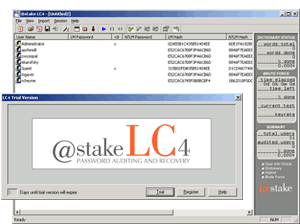
\includegraphics[width=8cm]{images/lc4_splash.png}}
\end{center}

\begin{alltt}
\small
Consider that at one of the largest technology companies, where policy
required that passwords exceed 8 characters, mix cases, and include
numbers or symbols...

L0phtCrack obtained 18\% of the passwords in 10 minutes
90\% of the passwords were recovered within 48 hours on a Pentium II/300
The Administrator and most Domain Admin passwords were cracked
\link{http://www.atstake.com/research/lc/}
\end{alltt}

\slide{Pass the hash}

Lots of tools in pentesting pass the hash, reuse existing credentials and tokens
\emph{Still Passing the Hash 15 Years Later}
\link{http://passing-the-hash.blogspot.dk/2013/04/pth-toolkit-for-kali-interim-status.html}

\begin{quote}
If a domain is built using only modern Windows OSs and COTS products (which know how to operate within these new constraints), and configured correctly with no shortcuts taken, then these protections represent a big step forward.
\end{quote}

Source:\\
{\small\link{http://www.harmj0y.net/blog/penetesting/pass-the-hash-is-dead-long-live-pass-the-hash/}
\link{https://samsclass.info/lulz/pth-8.1.htm}}


\slide{Cain og Abel}

%\hlkimage{10cm}{cain_brute_attack.jpg}
\hlkimage{20cm}{cain-win.png}

\begin{list1}
\item  Cain og Abel anbefales   \link{http://www.oxid.it}
\end{list1}

\slide{John the ripper}

\begin{quote}
John the Ripper is a fast password cracker, currently available for
many flavors of Unix (11 are officially supported, not counting
different architectures), Windows, DOS, BeOS, and OpenVMS. Its primary
purpose is to detect weak Unix passwords. Besides several crypt(3)
password hash types most commonly found on various Unix flavors,
supported out of the box are Kerberos AFS and Windows NT/2000/XP/2003
LM hashes, plus several more with contributed patches.
\end{quote}

\begin{list1}
\item UNIX passwords kan knækkes med alec Muffets kendte Crack program
  eller eksempelvis John The Ripper \link{http://www.openwall.com/john/}
\end{list1}



\slide{Cracking passwords}

\begin{list2}
\item Hashcat is the world's fastest CPU-based password recovery tool.
\item oclHashcat-plus is a GPGPU-based multi-hash cracker using a brute-force attack (implemented as mask attack), combinator attack, dictionary attack, hybrid attack, mask attack, and rule-based attack.
\item oclHashcat-lite is a GPGPU cracker that is optimized for cracking performance. Therefore, it is limited to only doing single-hash cracking using Markov attack, Brute-Force attack and Mask attack.
\item John the Ripper password cracker old skool men stadig nyttig
\end{list2}

Source:\\
\link{http://hashcat.net/wiki/}\\
\link{http://www.openwall.com/john/}


\slide{Parallella John}

\hlkimage{20cm}{parallella-john.png}

\link{https://twitter.com/solardiz/status/492037995080712192}

Warning: FPGA hacking - not finished part of presentation

\slide{Stacking Parallella boards}
\hlkimage{16cm}{4BoardStack.jpg}

\link{http://www.parallella.org/power-supply/}

\demo{Playtime - speed test openssl speed, John speed}

\demo{Cain/Abel, hashcat or John the Ripper }

30-40 minute testing

Grab hashes from \link{https://hashcat.net/wiki/doku.php?id=example_hashes}


\slide{Passwords vælges ikke tilfældigt}

\hlkimage{20cm}{50-most-used-passwords.png}

Source:
\link{https://wpengine.com/unmasked/}


\slide{Encryption key length}

\hlkimage{12cm}{encryption-crack.png}

Source: \link{http://www.mycrypto.net/encryption/encryption_crack.html}

More up to date:\\
In 1998, the EFF built Deep Crack for less than \$250,000\\
\link{https://en.wikipedia.org/wiki/EFF_DES_cracker}\\
FPGA Based UNIX Crypt Hardware Password Cracker\\
\link{http://www.sump.org/projects/password/}

\slide{WPA cracking med Pyrit}

\begin{quote}
\emph{Pyrit} takes a step ahead in attacking WPA-PSK and WPA2-PSK, the protocol that today de-facto protects public WIFI-airspace. The project's goal is to estimate the real-world security provided by these protocols. Pyrit does not provide binary files or wordlists and does not encourage anyone to participate or engage in any harmful activity. {\bf This is a research project, not a cracking tool.}

\emph{Pyrit's} implementation allows to create massive databases, pre-computing part of the WPA/WPA2-PSK authentication phase in a space-time-tradeoff. The performance gain for real-world-attacks is in the range of three orders of magnitude which urges for re-consideration of the protocol's security. Exploiting the computational power of GPUs, \emph{Pyrit} is currently by far the most powerful attack against one of the world's most used security-protocols.
\end{quote}

\begin{list1}
\item \link{http://pyrit.wordpress.com/about/}
\item Also check out the Reaver brute force WPS\\ \link{https://code.google.com/p/reaver-wps/}
\end{list1}

\slide{ Wi-Fi Protected Setup, WPS hacking - Reaver}

\begin{quote}
How Reaver Works
Now that you've seen how to use Reaver, let's take a quick overview of how Reaver works. The tool takes advantage of a vulnerability in something called Wi-Fi Protected Setup, or WPS. It's a feature that exists on many routers, intended to provide an easy setup process, and it's tied to a PIN that's hard-coded into the device. Reaver exploits a flaw in these PINs; the result is that, with enough time, it can reveal your WPA or WPA2 password.
\end{quote}

\centerline{Hvad betyder ease of use?}

Source: \\
\link{https://code.google.com/p/reaver-wps/}\\
{\footnotesize \link{http://lifehacker.com/5873407/how-to-crack-a-wi+fi-networks-wpa-password-with-reaver}}

\slide{WPS Design Flaws used by Reaver }

\hlkimage{22cm}{wps-design-flaw-1.png}

\centerline{Pin only, no other means necessary}

Source:\\
\link{http://sviehb.files.wordpress.com/2011/12/viehboeck_wps.pdf}



\slide{WPS Design Flaws used by Reaver }

\hlkimage{14cm}{wps-design-flaw-2.png}

\centerline{Reminds me of NTLM cracking, crack parts independently}

Source:\\
\link{http://sviehb.files.wordpress.com/2011/12/viehboeck_wps.pdf}



\slide{Are your data secure - data at rest}

\hlkimage{15cm}{images/data-integrity-1.pdf}

\begin{list1}
\item Stolen laptop, tablet, phone - can anybody read your data?
\item Do you trust "remote wipe"
\item How do you in fact wipe data securely off devices, and SSDs?
\item Encrypt disk and storage devices before using them in the first place!
\end{list1}


\slide{Circumvent security - single user mode boot}
\begin{list1}
\item Unix systems often allows boot into singleuser mode\\
press command-s when booting Mac OS X
\item Laptops can often be booted using PXE network or CD boot
\item Mac computers can become a Firewire disk\\
hold t when booting - firewire target mode
\item Unrestricted access to un-encrypted data
\item Moving hard drive to another computer is also easy
\end{list1}
\pause
\centerline{Physical access is often - {\bf game over}}


\slide{Encrypting hard disk}

\hlkimage{14cm}{images/apple-filevault.png}

\begin{list1}
\item Becoming available in the most popular client operating systems
\begin{list2}
\item Microsoft Windows Bitlocker - requires Ultimate or Enterprise
\item Apple Mac OS X - FileVault og FileVault2
\item FreeBSD GEOM og GBDE - encryption framework
\item Linux LUKS distributions like Ubuntu ask to encrypt home dir during installation
\item PGP disk - Pretty Good Privacy - makes a virtuel krypteret disk
\item TrueCrypt - similar to PGP disk, a virtual drive with data, cross platform
\item Some vendors have BIOS passwords, or disk passwords
\end{list2}
\end{list1}



\slide{Attacks on disk encryption}

\begin{list1}
\item Firewire, DMA \& Windows, Winlockpwn via FireWire\\
Hit by a Bus: Physical Access Attacks with Firewire Ruxcon 2006
\vskip 5mm
\item Removing memory from live system - data is not immediately lost, and can be read under some circumstances\\
Lest We Remember: Cold Boot Attacks on Encryption Keys\\
\link{http://citp.princeton.edu/memory/}
\item This is very CSI or Hollywoord like - but a real threat
\item VileFault decrypts encrypted Mac OS X disk image files\\ \link{https://code.google.com/p/vilefault/}

\item  FileVault Drive Encryption (FVDE) (or FileVault2) encrypted volumes\\
\link{https://code.google.com/p/libfvde/}
\end{list1}

\centerline{So perhaps use both hard drive encryption AND turn off computer after use?}

\slide{... and deleting data}

\hlkimage{14cm}{dban-screenshot.png}

\begin{list1}
\item Getting rid of data from old devices is a pain
\item Some tools will not overwrite data, leaving it vulnerable to recovery
\item Even secure erase programs might not work on SSD - due to reallocation of blocks
\item I have used Darik's Boot and Nuke ("DBAN") \link{http://www.dban.org/}
\end{list1}





\slide{Backup}

\vskip 3cm
\centerline{\LARGE \bf Kom igang!}

\begin{list2}
\item Skriv på DVD - DVD brændere i mange laptops idag
\item Gem på netværket - Dropbox, husk en yderligere backup!
\item Brug Duplicity på egen server, eller tilsvarende services
\end{list2}

Mat Honan epic hacking :-(\\ {\small\link{http://www.wired.com/gadgetlab/2012/08/apple-amazon-mat-honan-hacking/all/}}

Ransomware er hot topic i 2015 :-(


\slide{Duplicity}

\begin{quote}
{\large\bf What is it?}

Duplicity backs directories by producing encrypted tar-format volumes and uploading them to a remote or local file server. Because duplicity uses librsync, the incremental archives are space efficient and only record the parts of files that have changed since the last backup. Because duplicity uses {\bf GnuPG} to encrypt and/or sign these archives, they will be safe from spying and/or modification by the server.
\end{quote}

\link{http://duplicity.nongnu.org/} duplicity home page

\link{http://www.gnupg.org/} The GNU Privacy Guard


\slide{VPN}

\hlkimage{12cm}{openvpn-gui-systray.png}

\begin{list1}
\item Virtual Private Networks are useful - or even required when travelling
\item VPN \link{http://en.wikipedia.org/wiki/Virtual_private_network}
\item SSL/TLS VPN - Multiple incompatible vendors: OpenVPN, Cisco, Juniper, F5 Big IP
\item IETF IPsec does work cross-vendors - sometimes, and is also increasingly becoming blocked or unusable due to NAT :-(
\item Recommended starting point OpenVPN - free and open, clients for "anything"
\end{list1}

\slide{IPsec IKE-SCAN}

Scan IPs for VPN endpoints with ike-scan:
\begin{alltt}\small
root@kali:~# ike-scan 91.102.91.30
Starting ike-scan 1.9 with 1 hosts
(http://www.nta-monitor.com/tools/ike-scan/)
91.102.91.30	Notify message 14 (NO-PROPOSAL-CHOSEN)
HDR=(CKY-R=f0d6043badb2b7bc, msgid=f97a7508)

Ending ike-scan 1.9: 1 hosts scanned in 1.238 seconds (0.81 hosts/sec).
0 returned handshake; 1 returned notify
\end{alltt}

Source:\\
{\small\link{http://www.nta-monitor.com/tools-resources/security-tools/ike-scan}}

crack IKE psk?\\
\link{http://ikecrack.sourceforge.net/} \\
\link{https://www.trustwave.com/Resources/SpiderLabs-Blog/Cracking-IKE-Mission-Improbable-(Part-1)/}

\slide{ike-scan network scanning}

\begin{alltt}\small
hlk@cornerstone03:~$ sudo ike-scan -M 91.102.91.0/24
Starting ike-scan 1.9 with 256 hosts
(http://www.nta-monitor.com/tools/ike-scan/)
91.102.91.14	Notify message 14 (NO-PROPOSAL-CHOSEN)
	HDR=(CKY-R=94dd41cf44da082b, msgid=602c35c1)
91.102.91.30	Notify message 14 (NO-PROPOSAL-CHOSEN)
	HDR=(CKY-R=e21e89d16f898aa5, msgid=ff41d51c)
91.102.91.70	Notify message 14 (NO-PROPOSAL-CHOSEN)
	HDR=(CKY-R=e882d9b4477b847b, msgid=55be4339)
91.102.91.78	Notify message 14 (NO-PROPOSAL-CHOSEN)
	HDR=(CKY-R=1fc54d8c3042daa3, msgid=ea705f39)
91.102.91.150	Notify message 14 (NO-PROPOSAL-CHOSEN)
	HDR=(CKY-R=d5470f881de6d2d9, msgid=2bf5f5ef)
91.102.91.158	Notify message 14 (NO-PROPOSAL-CHOSEN)
	HDR=(CKY-R=9f7af04bcb0152a9, msgid=44f26f01)

Ending ike-scan 1.9: 256 hosts scanned in 40.465 seconds (6.33 hosts/sec).
0 returned handshake; 6 returned notify
\end{alltt}



\slide{Multiple browsers}

\hlkimage{20cm}{multi-browser-strategy.png}

\begin{list2}
\item Strict Security settings in the general browser, Firefox or Chrome?
\item More lax security settings for "trusted sites" - like home banking
\item Security plugins like HTTPS Everywhere and NoScripts for generic browsing
\end{list2}

\slide{HTTPS Everywhere}

\hlkimage{5cm}{HTTPS_Everywhere_new_logo.jpg}
\begin{quote}
HTTPS Everywhere is a Firefox extension produced as a collaboration between The Tor Project and the Electronic Frontier Foundation. It encrypts your communications with a number of major websites.
\end{quote}

\centerline{\link{http://www.eff.org/https-everywhere}}

\slide{DNSSEC trigger}

\hlkimage{7cm}{dnssec-trigger.png}

Lots of DNSSEC tools, I recommend DNSSEC-trigger a local name server for your laptop

\begin{list2}
\item DNSSEC Validator for firefox\\ \link{https://addons.mozilla.org/en-us/firefox/addon/dnssec-validator/}
\item OARC tools \link{https://www.dns-oarc.net/oarc/services/odvr}
\item \link{http://www.nlnetlabs.nl/projects/dnssec-trigger/}
\end{list2}

\slide{DNSSEC NSEC walk the zone}

\begin{quote}
DNSSEC:NSEC vs. NSEC3

The Domain Name System Security Extensions(DNSSEC) provide two different records for securely handling non-existent names in DNS, NSEC and NSEC3. They are mutually exclusive, so operators need to pick one when deploying DNSSEC.

The problem both NSEC and NSEC3 solve is knowing when a name exists within a given zone. This is required to prevent malicious actors from sending fake negative responses to queries.

... the challenge with the plain NSEC record is that someone could use the NSEC responses to “walk the zone” and build a list of all of the records in a DNS zone.
\end{quote}

Source:\\
{\small\link{http://www.internetsociety.org/deploy360/resources/dnssec-nsec-vs-nsec3/}}

Perhaps try \link{http://josefsson.org/walker/}


\slide{DANE}

\begin{quote}
Objective:

Specify mechanisms and techniques that allow Internet applications to
establish cryptographically secured communications by using information
distributed through DNSSEC for discovering and authenticating public
keys which are associated with a service located at a domain name.
\end{quote}

DNS-based Authentication of Named Entities (dane)\\
\link{https://datatracker.ietf.org/wg/dane/charter/}\\
{\footnotesize \link{http://googleonlinesecurity.blogspot.dk/2011/04/improving-ssl-certificate-security.html}}

\vskip 2cm

\centerline{\Large DNSSEC er ved at være godt udbredt - undtagen i DK}
(findes på .dk zonen, men næsten ingen resolvere)

\slide{www.uncensoreddns.org}

\hlkimage{17cm}{censurfridns-1.png}

\slide{Konklusion: Kryptografi er svært}

%Stoler vi på de andre autentificeringsmetoder?}
\hlkimage{20cm}{crypto-class.png}

Åbent kursus på Stanford\\
\link{http://crypto-class.org/}

\slide{Kryptering: Cryptography Engineering}

\hlkimage{8cm}{book-ce-150w.jpg}

\emph{Cryptography Engineering} by
Niels Ferguson, Bruce Schneier, and Tadayoshi Kohno
\link{https://www.schneier.com/book-ce.html}

\centerline{Kryptering sikrer fortrolighed og integritet af beskederne}


\slide{24 Deadly Sins of Software Security}

\hlkrightimage{5cm}{24-deadly.jpg}
\emph{24 Deadly Sins of Software Security} af Michael Howard, David Leblanc, John Viega 2009

\begin{list1}
\item {\bf Obligatorisk læsning for alle udviklere}
\item Denne bog er præcis og giver overblik på kun 432 sider
\item Buffer Overruns, Format String Problems, Integer Overflows, SQL Injection, Command Injection,
Failing to Handle Errors, Cross-Site Scripting, Failing to Protect Network Traffic, Magic URLs Hidden Form Fields,
Improper Use of SSL and TLS, Weak Password-Based Systems, Failing to Store and Protect Data Securely, Information
Leakage, Improper File Access, Trusting Network Name Resolution, Race Conditions, Unauthenticated Key Exchange, Cryptographically Strong Random Numbers, Poor Usability
\end{list1}


\slide{Open Mike night ...}

\vskip 3 cm

\centerline{\Large Hvad glemte jeg? Kom med dine favoritter \smiley}

evalg, DNS censur, NemID bashing, malware sucks, Android malware, iPhone malware?

Did you notice how a lot of the links in this presentation uses HTTPS - encrypted


\myquestionspage

\end{document}
